
\renewcommand{\tmpwidth}{0.14\linewidth}
\setlength{\tabcolsep}{1pt}
\begin{figure*}[!ht]
    \centering
    \begin{tabular}{c c c c c c c}

	% \includegraphics[width=\tmpwidth]{figures/editing/000143_to130_0020_input.png} & 
	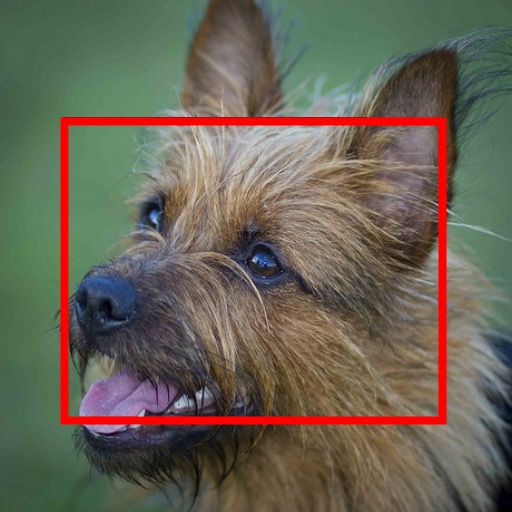
\includegraphics[width=\tmpwidth]{figures/editing/000193_to282_0006_input.png} &
	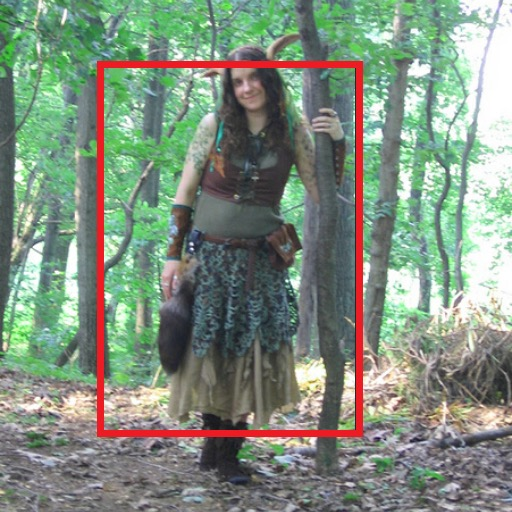
\includegraphics[width=\tmpwidth]{figures/editing/000689_to282_0000_input.png} &
	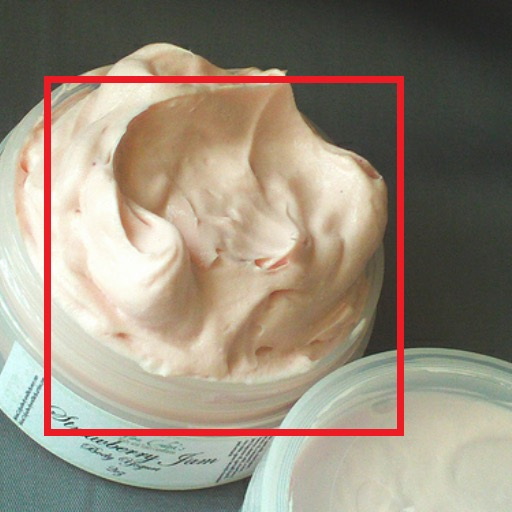
\includegraphics[width=\tmpwidth]{figures/editing/000838_to282_0004_input.png} &
	\includegraphics[width=\tmpwidth]{figures/editing/000538_to282_0024_input.png} &
	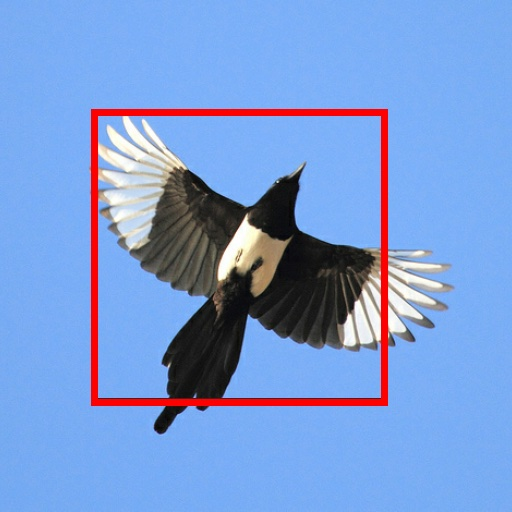
\includegraphics[width=\tmpwidth]{figures/editing/000018_to282_0002_input.png} &
	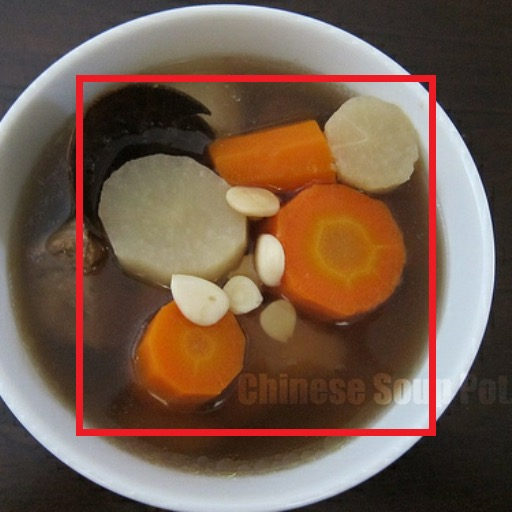
\includegraphics[width=\tmpwidth]{figures/editing/000809_to282_0002_input.png} &
	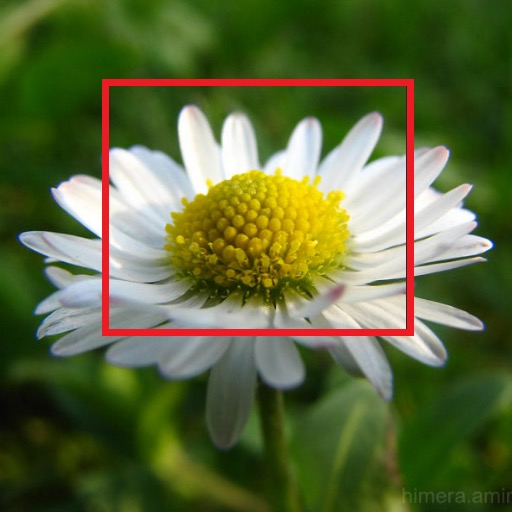
\includegraphics[width=\tmpwidth]{figures/editing/000985_to282_0000_0024_input.png} 
    \\ 
	% \includegraphics[width=\tmpwidth]{figures/editing/000143_to130_0020_output.png} & 
	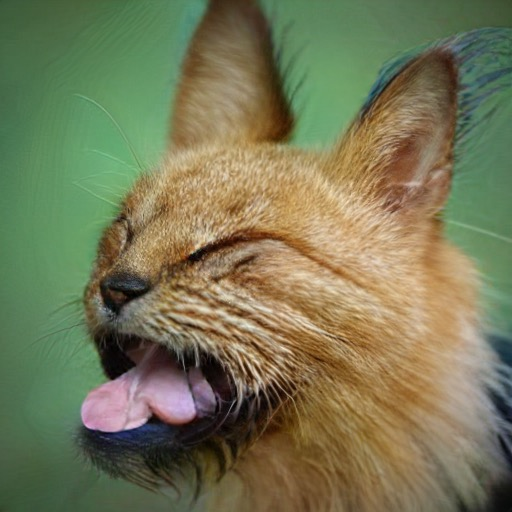
\includegraphics[width=\tmpwidth]{figures/editing/000193_to282_0006_output.png} &
	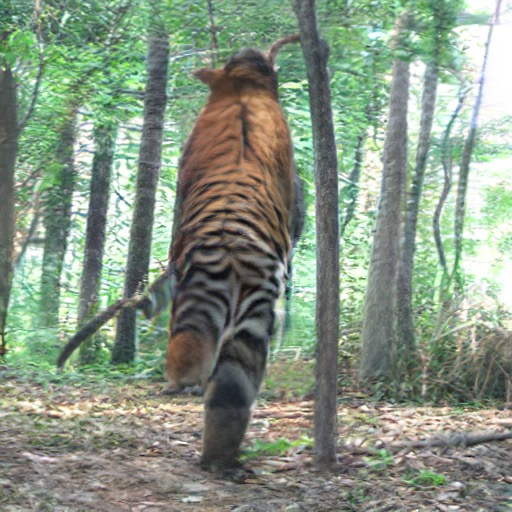
\includegraphics[width=\tmpwidth]{figures/editing/000689_to282_0000_output.png} &
	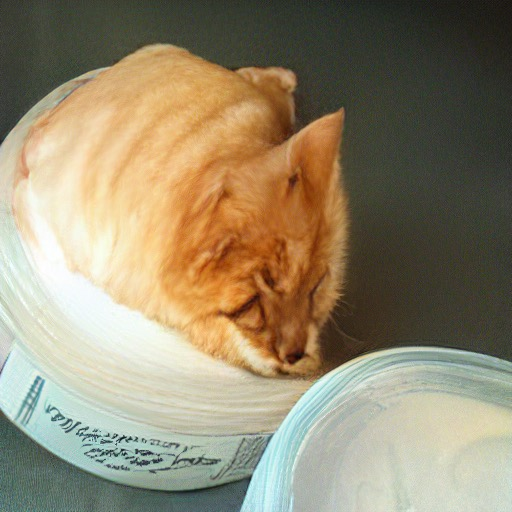
\includegraphics[width=\tmpwidth]{figures/editing/000838_to282_0004_output.png} &
    \includegraphics[width=\tmpwidth]{figures/editing/000538_to282_0036_output.png} &
    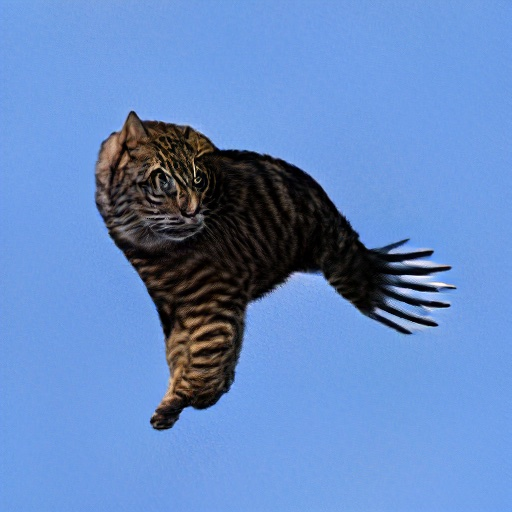
\includegraphics[width=\tmpwidth]{figures/editing/000018_to282_0000_output.png} &
	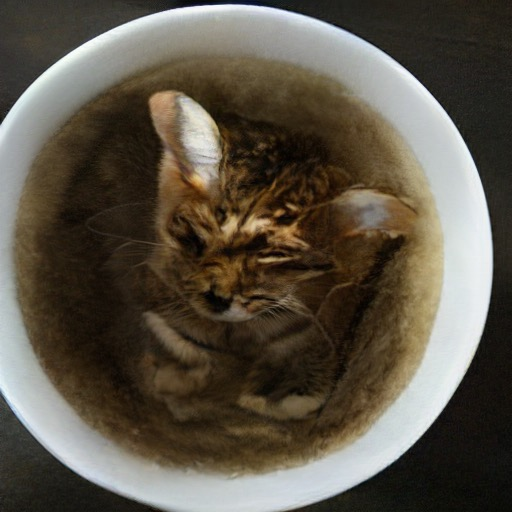
\includegraphics[width=\tmpwidth]{figures/editing/000809_to282_0002_output.png} &
    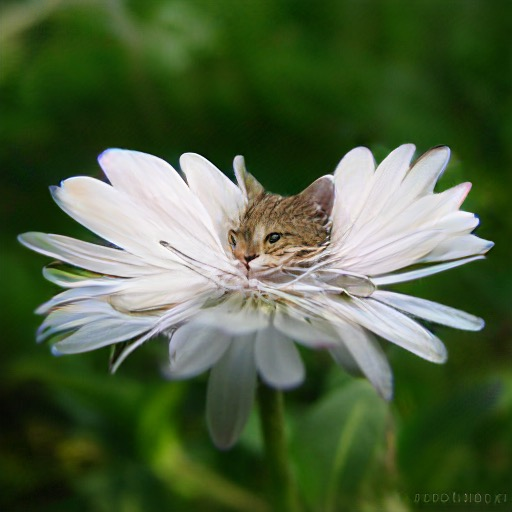
\includegraphics[width=\tmpwidth]{figures/editing/000985_to282_0000_0012_output.png} 
    \\
    \end{tabular}
    \caption{\textbf{Object modification.} Given input images in the first row, and a target class "tiger cat", \model replaces the bounding boxed regions with tiger cats. The fact that the synthesized tiger cat blends in with the rest of the image seamlessly highlights the composition ability of our model.  \todo{add bounding box}}
    \vspace{-6mm}
    \label{fig:editing}
\end{figure*}